% !TeX root = ../HebutThesis_example.tex(此文件是被HebutThesis_example.tex调用的)
\chapter{绪论}
\setcounter{page}{1}
\pagenumbering{arabic}



\section{标题1}
%另起一行在生成的pdf中不会有影响,需要另起一段时请空一行空行。

绪论:
绪论相当于论文的开头,它是三段式论文的第一段(后二段是本论和结论。
绪论与摘要写法不完全相同,摘要要写得高度概括、简略,绪论可以稍加具体一些,文字以1000字左右为宜。
绪论一般应包括以下几个内容:

1 为什么要写这篇论文,要解决什么问题,主要观点是什么。
2 对本论文研究主题范围内已有文献的评述(包括与课题相关的历史的回顾,资料来源、性质及运用情况等)。
3 说明本论文所要解决的问题,所采用的研究手段、方式、方法。明确研究工作的界限和规模。
4 概括论文的主要工作内容。
\section{标题2}

\subsection{插图}
插图:一般情况下,在正文中,先见到图号和图的内容再展示图。
特殊情况须延后的插图不应跨节。

通常使用的函数图采用简化形式,称为简写函数图,例如图{\ref{fig:historyhebut}}。
\begin{figure}[ht]
    \centering
    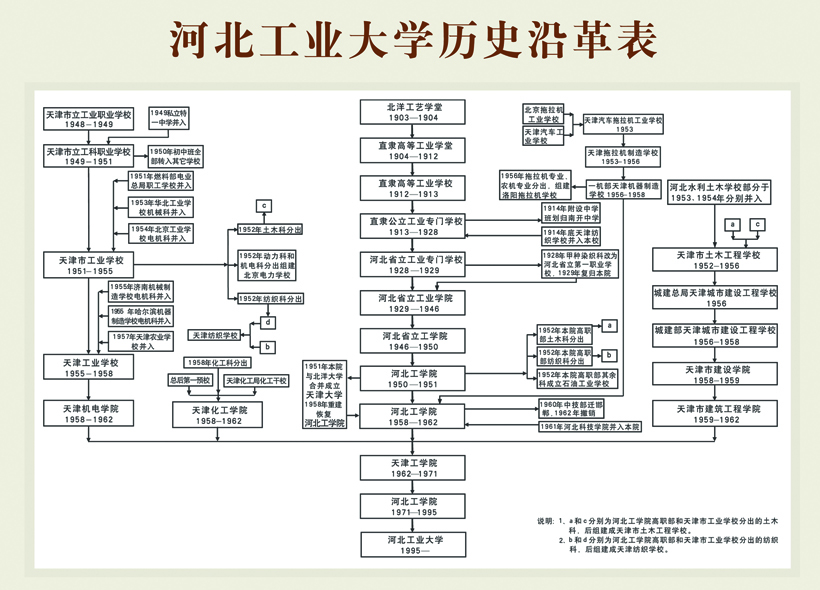
\includegraphics[width=\textwidth]{figures/historyhebut}
    \caption{河北工业大学历史沿革}\label{fig:historyhebut}
\end{figure}

\section{标题3}
引用如这样\cite{song_score-based_2020}
\section{标题4}


\subsection{插表}
一般情况下,表格须通栏,即表格宽度与正文版面平齐,如下表所示。
\begin{table}
    \centering
    \caption{测试用例表}\label{tab:table_centered}
    \begin{tabularx}{\textwidth}{>{\centering\arraybackslash}X>{\centering\arraybackslash}X>{\centering\arraybackslash}X}
    \toprule
    列1 & 列2 & 列3 \\
    \midrule
    有效 & 001 & 通过 \\
    无效 & 002 & 未通过 \\
    \bottomrule
    \end{tabularx}
\end{table}
